%Punchline!

Given the measured amounts of mixing described in Section \ref{sec:obs} and the reduced density ratios $r$ computed for stars of various masses and metallicities described in Section \ref{sec:mesa_results}, it is now possible to compare the observations to the predictions of various thermohaline models from Section \ref{sec:formalism} and to assess whether the observed mixing is qualitatively consistent with any such theoretical prescription.
%
We show in Figure \ref{Fig:punchline} the corrected changes in [C/N] compared to the inferred reduced density ratios on axes analogous to those of Figure \ref{fig:parameterization_compare}, where the y axis represented the rate of mixing. 
The four panels correspond to the four modeling configurations described in Section \ref{sec:mesa_experiment}. 

We first note that the observed trends are not strongly sensitive to the assumed 1D mixing model: mixing decreases with increasing reduced density ratio regardless of parameterization.
%
Besides this, there are similarities and differences between the data and the theoretical predictions, which are reproduced in Figure \ref{Fig:compare} for comparison. A key finding is that the observed mixing is strongly correlated with the fluid parameters as predicted; this is true for stars with different masses and metallicities but similar reduced density ratios.
We observe a decrease in the amount of mixing as the density ratio increases, which is consistent with standard 1D prescriptions of thermohaline mixing but inconsistent with the prescription from \citet{harrington}, which was informed by magnetohydrodynamic simulations. 
We also find that the range of average reduced density ratios probed by the observational data we have available here is much smaller than the range of density ratios simulated by and studied within the theoretical 3D fluid dynamics community \citep[e.g.][]{brown_etal_2013}, although we note that the full range of ratios do appear in each individual simulation (See Appendix \ref{app:movie}).

%FIGURE solar---------------------------------------------------
\begin{figure*}[!tb]
\begin{center}
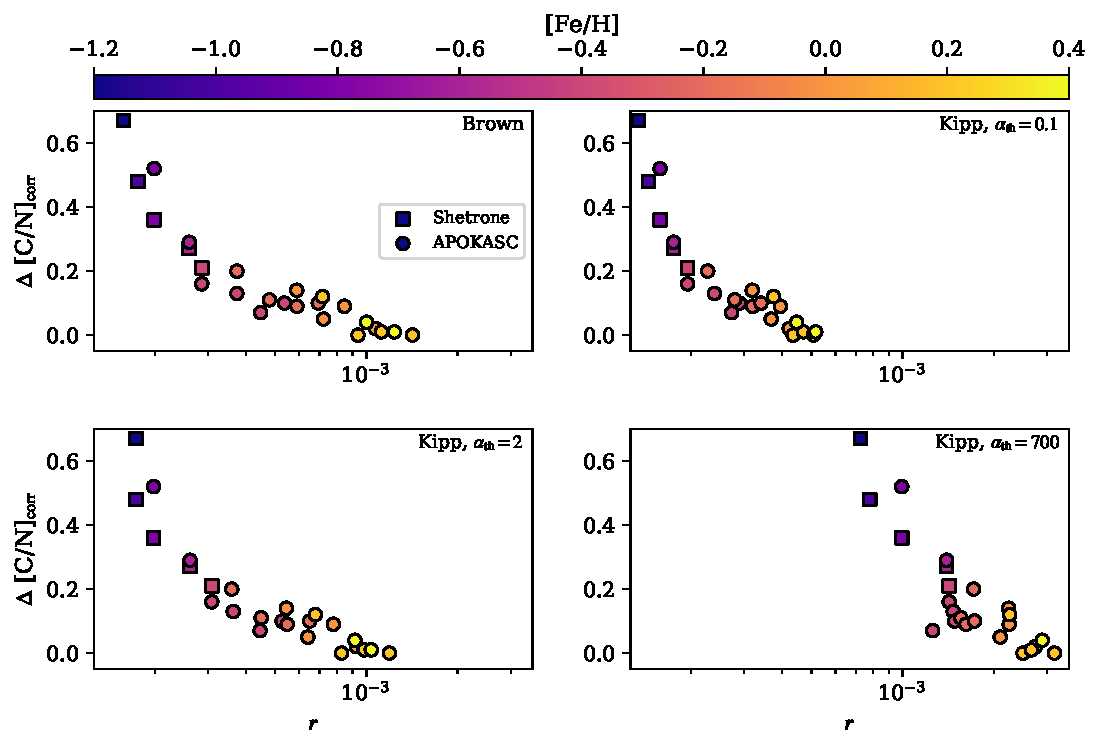
\includegraphics[width=\textwidth]{mixing_vs_r.pdf}%[width=9cm, clip=true, trim=1in 1in 1in 1in]{./Figs/omgcomp.eps}
\caption{Corrected measurements of the change in [C/N] near the red giant branch bump are compared to the reduced density ratio inferred from one-dimensional models using various thermohaline mixing prescriptions (Brown, Kippenhahn $\alpha_{\rm th}=0.1$, Kippenhahn $\alpha_{\rm th}=0.2$,Kippenhahn $\alpha_{\rm th}=0.700$). Observations are color coded by the metallicity bin of each data point. In general, there is a clear correlation between these parameters, suggesting that the observed mixing may indeed be related to
the unstable mean molecular weight gradient. Mixing and the reduced density ratio $r$ are inversely correlated, which is consistent with hydrodynamic thermohaline prescriptions. 
\label{Fig:punchline}
}
\end{center}
\end{figure*}

\begin{figure*}[!tb]
\begin{center}
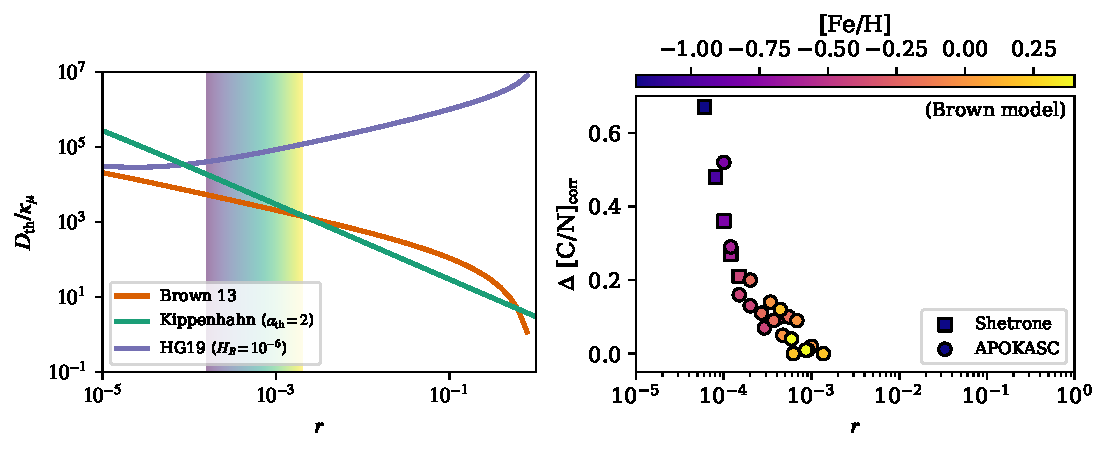
\includegraphics[width=\textwidth]{punchline.pdf}
\caption{\textbf{Left:} A reproduction of Figure \ref{fig:parameterization_compare} showing the predicted rate of mixing versus the reduced density ratio in various prescriptions of thermohaline mixing, including hydrodynamic (orange, green) and magnetohydrodynamic (purple) models. \textbf{Right:} The observed extra mixing near the red giant branch bump as a function of the reduced density ratio inferred from one dimensional stellar evolution models. While the conversion from the change in a mixing diagnostic to the fluid mixing rate is not trivial, and therefore we do not attempt it here, we note that the observed mixing amounts are strongly negatively correlated with $r$, with stars probing on average a relatively narrow range of the regime formally unstable to thermohaline mixing. }
\label{Fig:compare}
\end{center}
\end{figure*}


